\documentclass{article}
\usepackage[margin=0.4in, letterpaper]{geometry}
\usepackage{hyperref}
\usepackage{graphicx}
\usepackage{float}

\begin{document}
    \graphicspath{ {../plots/} }
    \listoffigures
    \section*{0000}
      \subsection*{test}
            \begin{figure}[H]
                \centering
                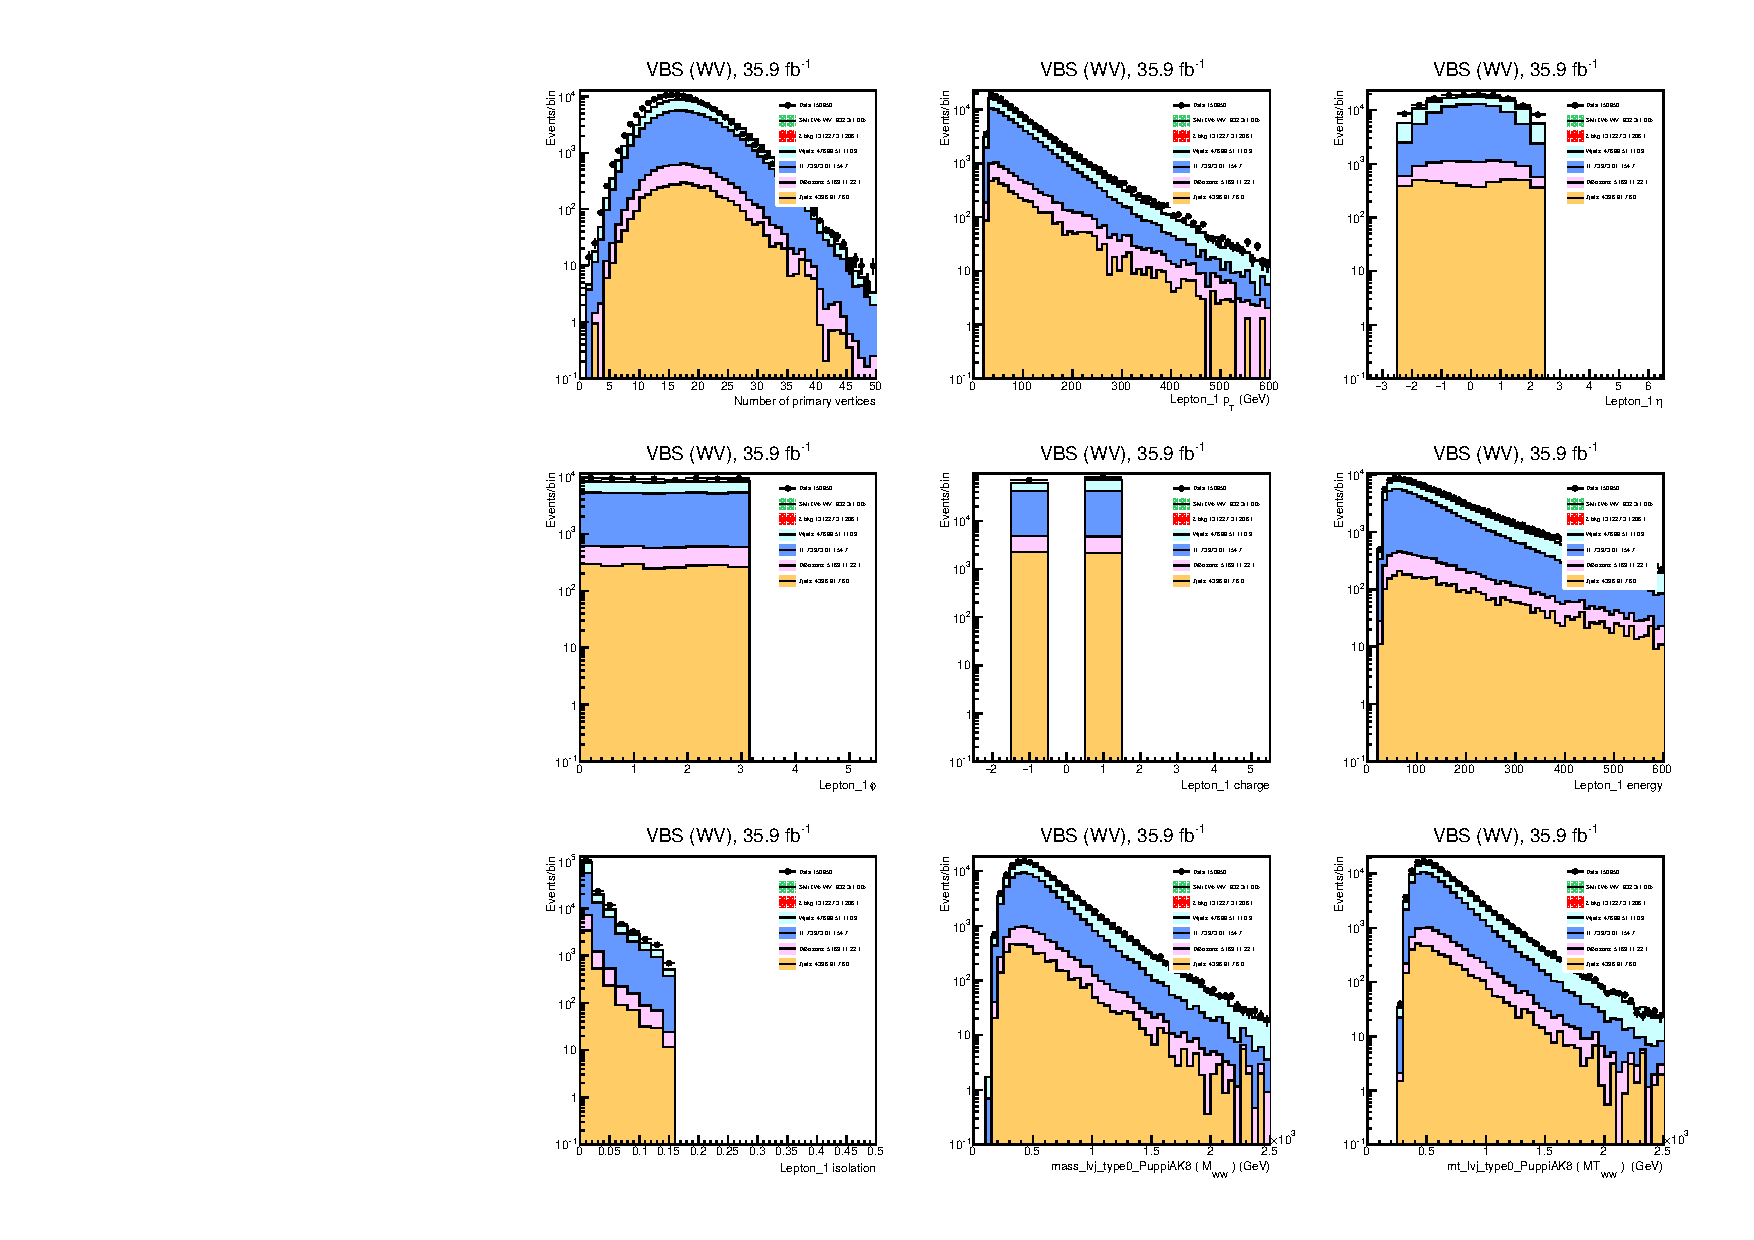
\includegraphics[width=\textwidth]{0000/c1_0000_test.pdf}
                \caption{0000 plot of c1 variables using cut: ``test"}
            \end{figure}
            \begin{figure}[H]
                \centering
                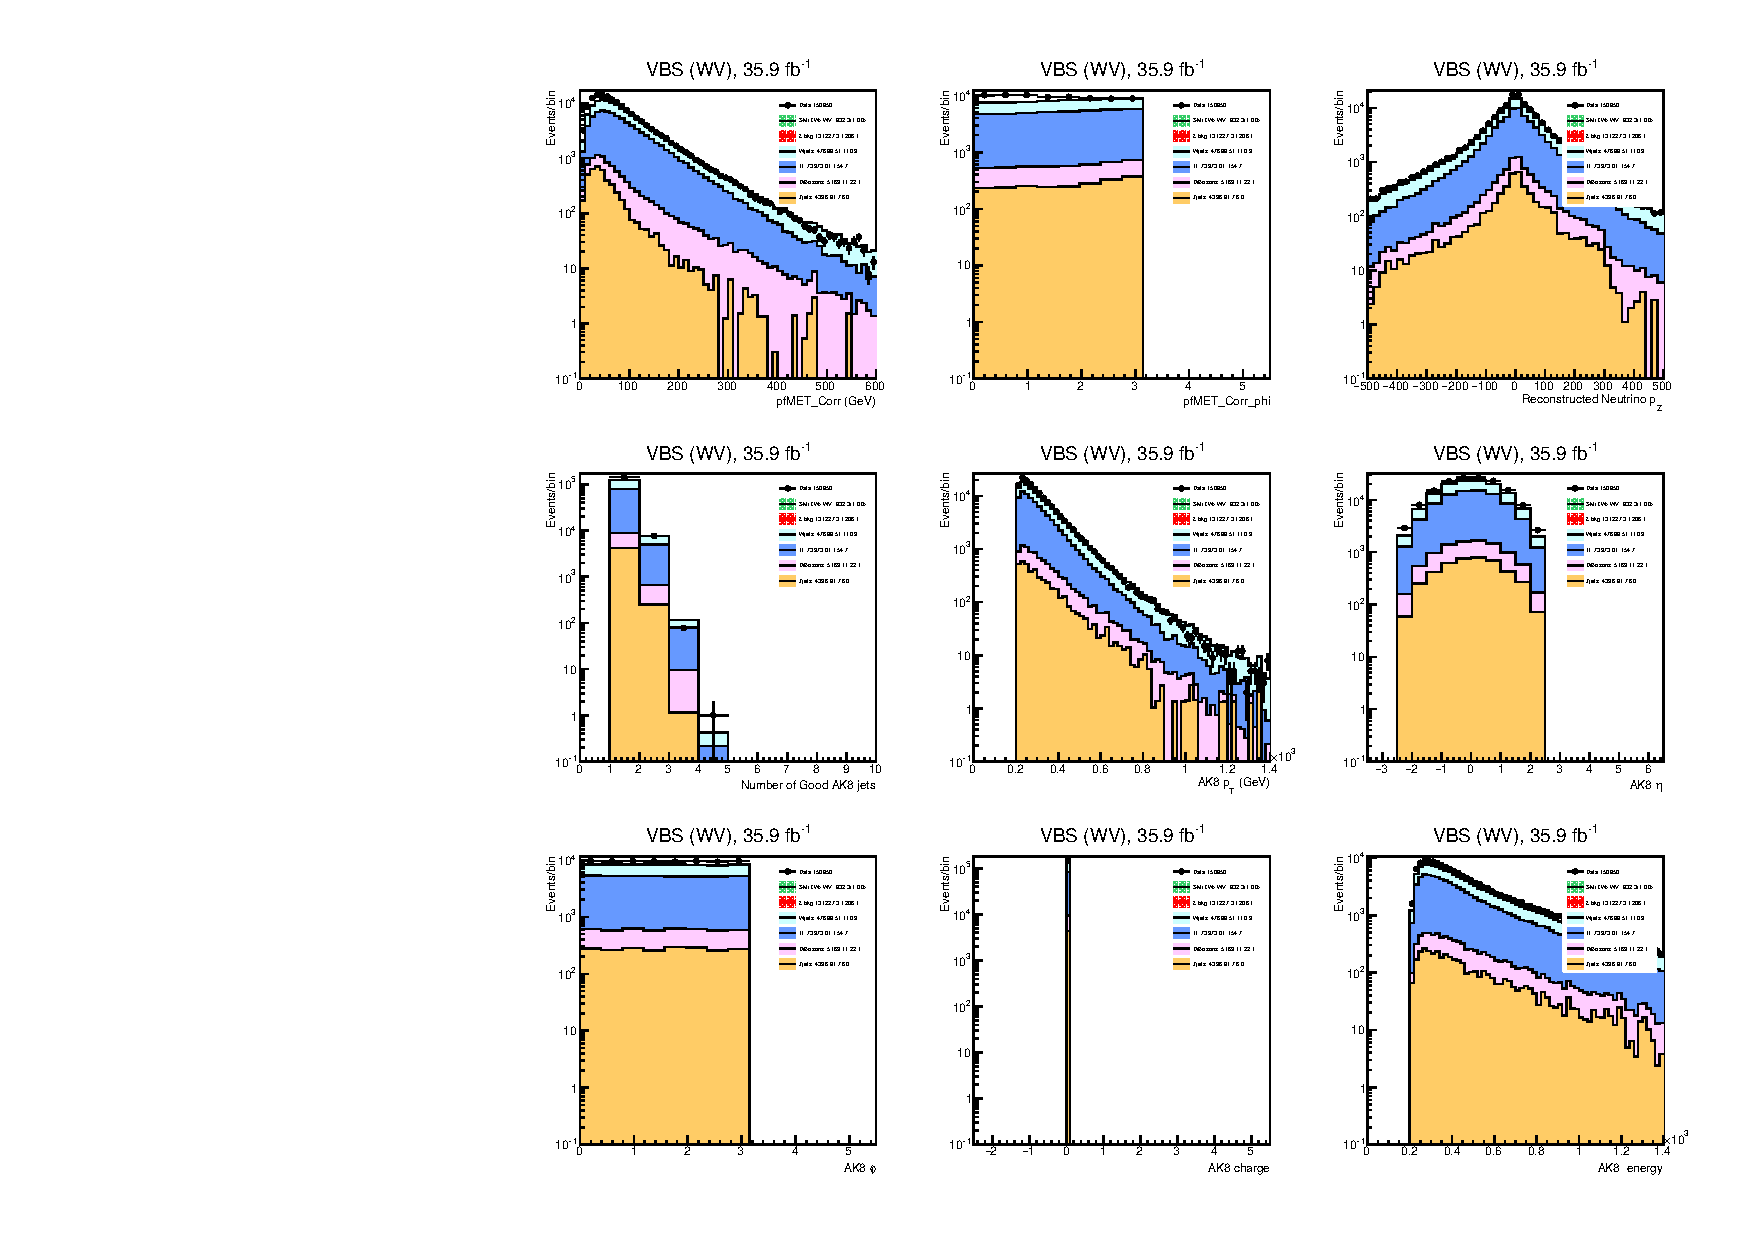
\includegraphics[width=\textwidth]{0000/c2_0000_test.pdf}
                \caption{0000 plot of c2 variables using cut: ``test"}
            \end{figure}
            \begin{figure}[H]
                \centering
                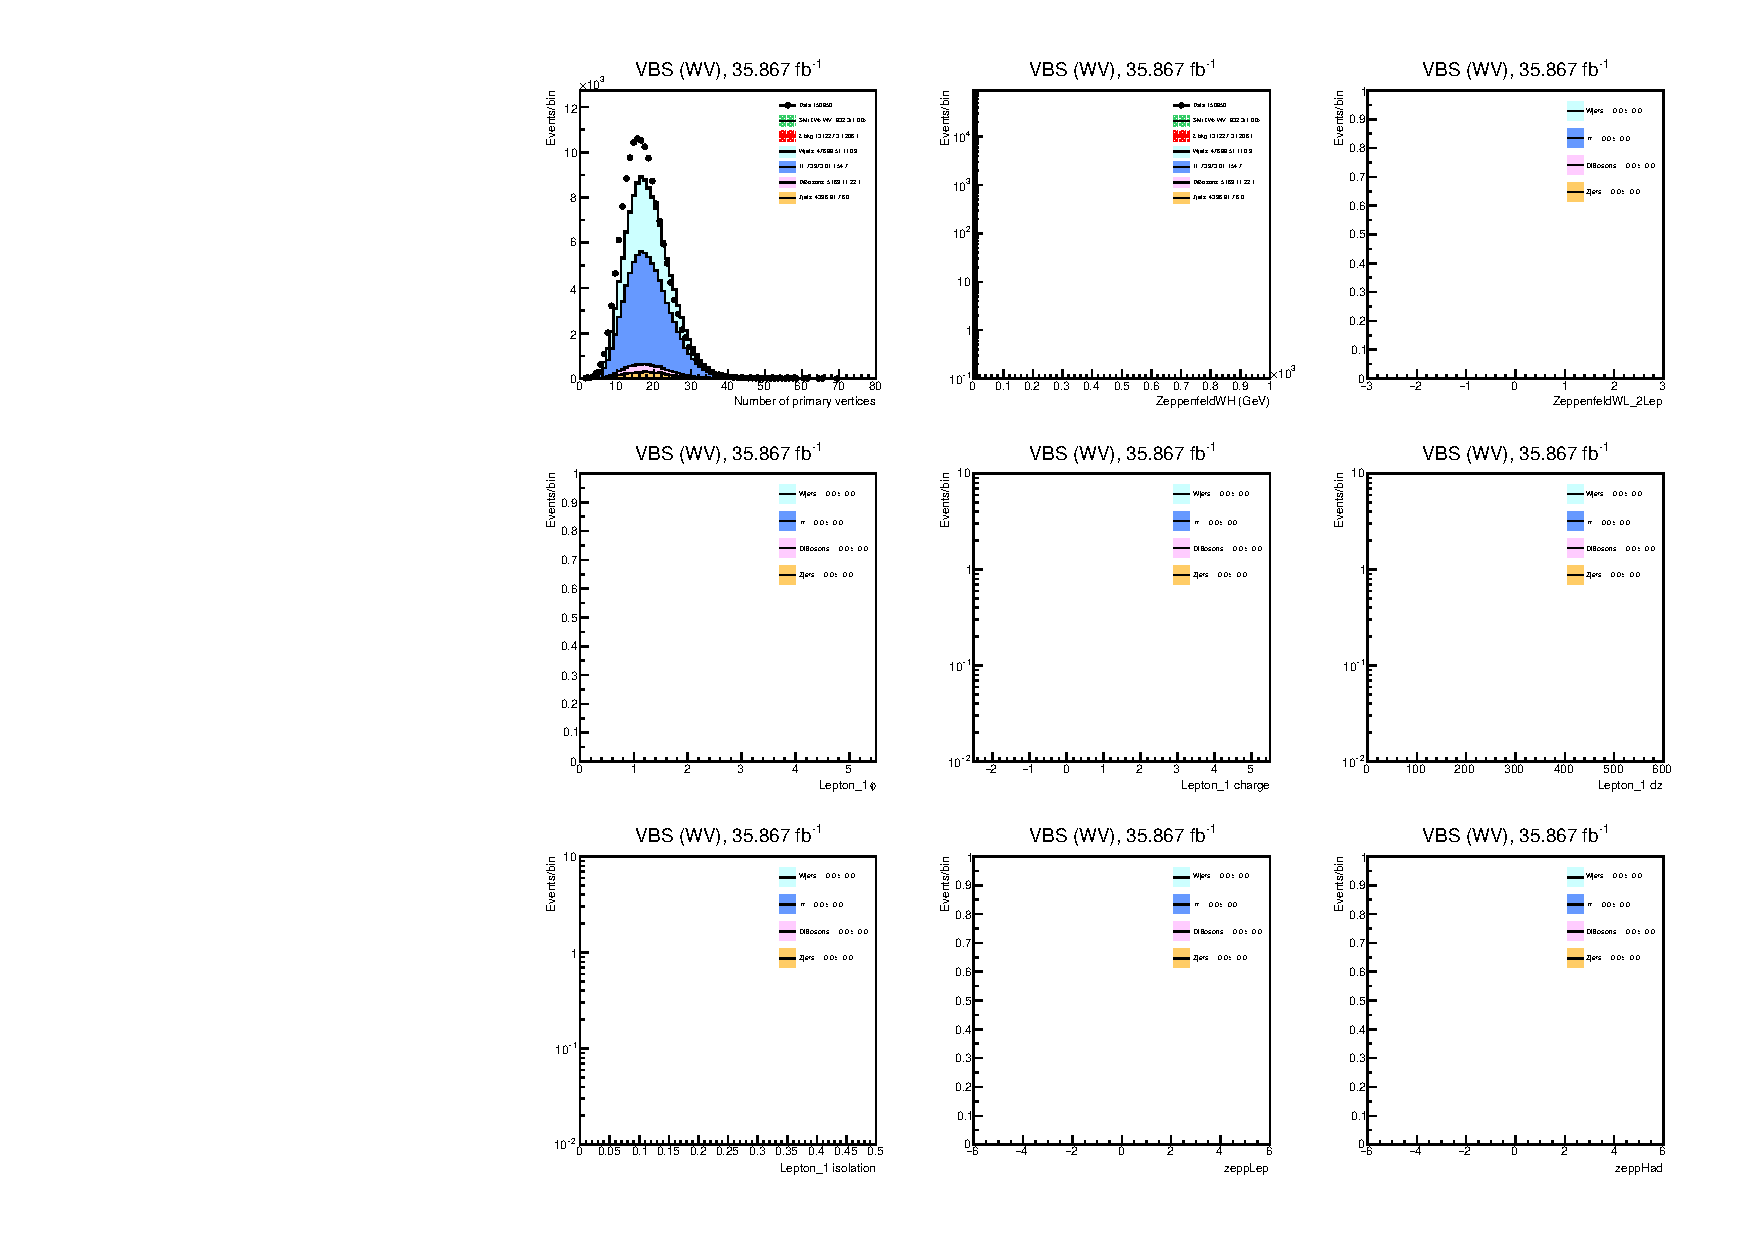
\includegraphics[width=\textwidth]{0000/c3_0000_test.pdf}
                \caption{0000 plot of c3 variables using cut: ``test"}
            \end{figure}
    \section*{2016}
      \subsection*{test}
            \begin{figure}[H]
                \centering
                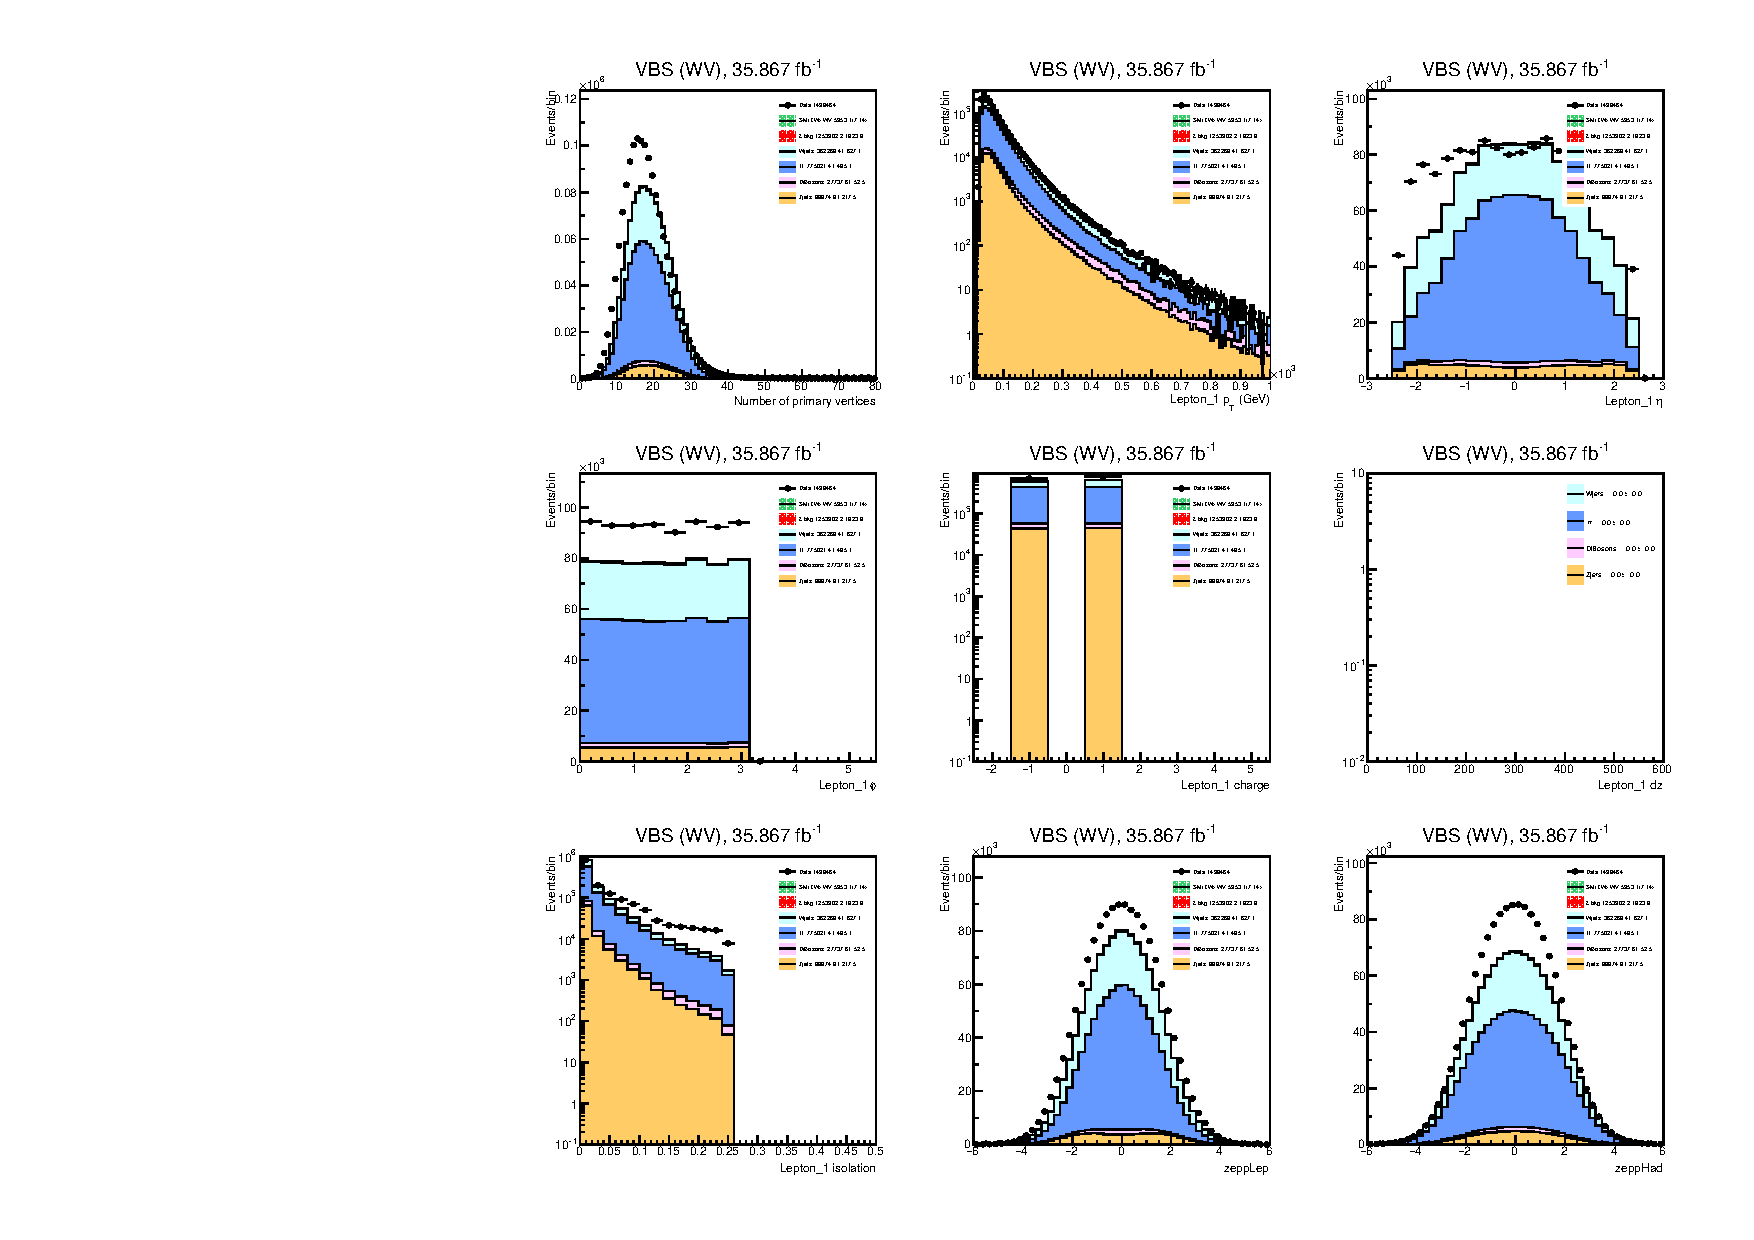
\includegraphics[width=\textwidth]{2016/c1_2016_test.pdf}
                \caption{2016 plot of c1 variables using cut: ``test"}
            \end{figure}
            \begin{figure}[H]
                \centering
                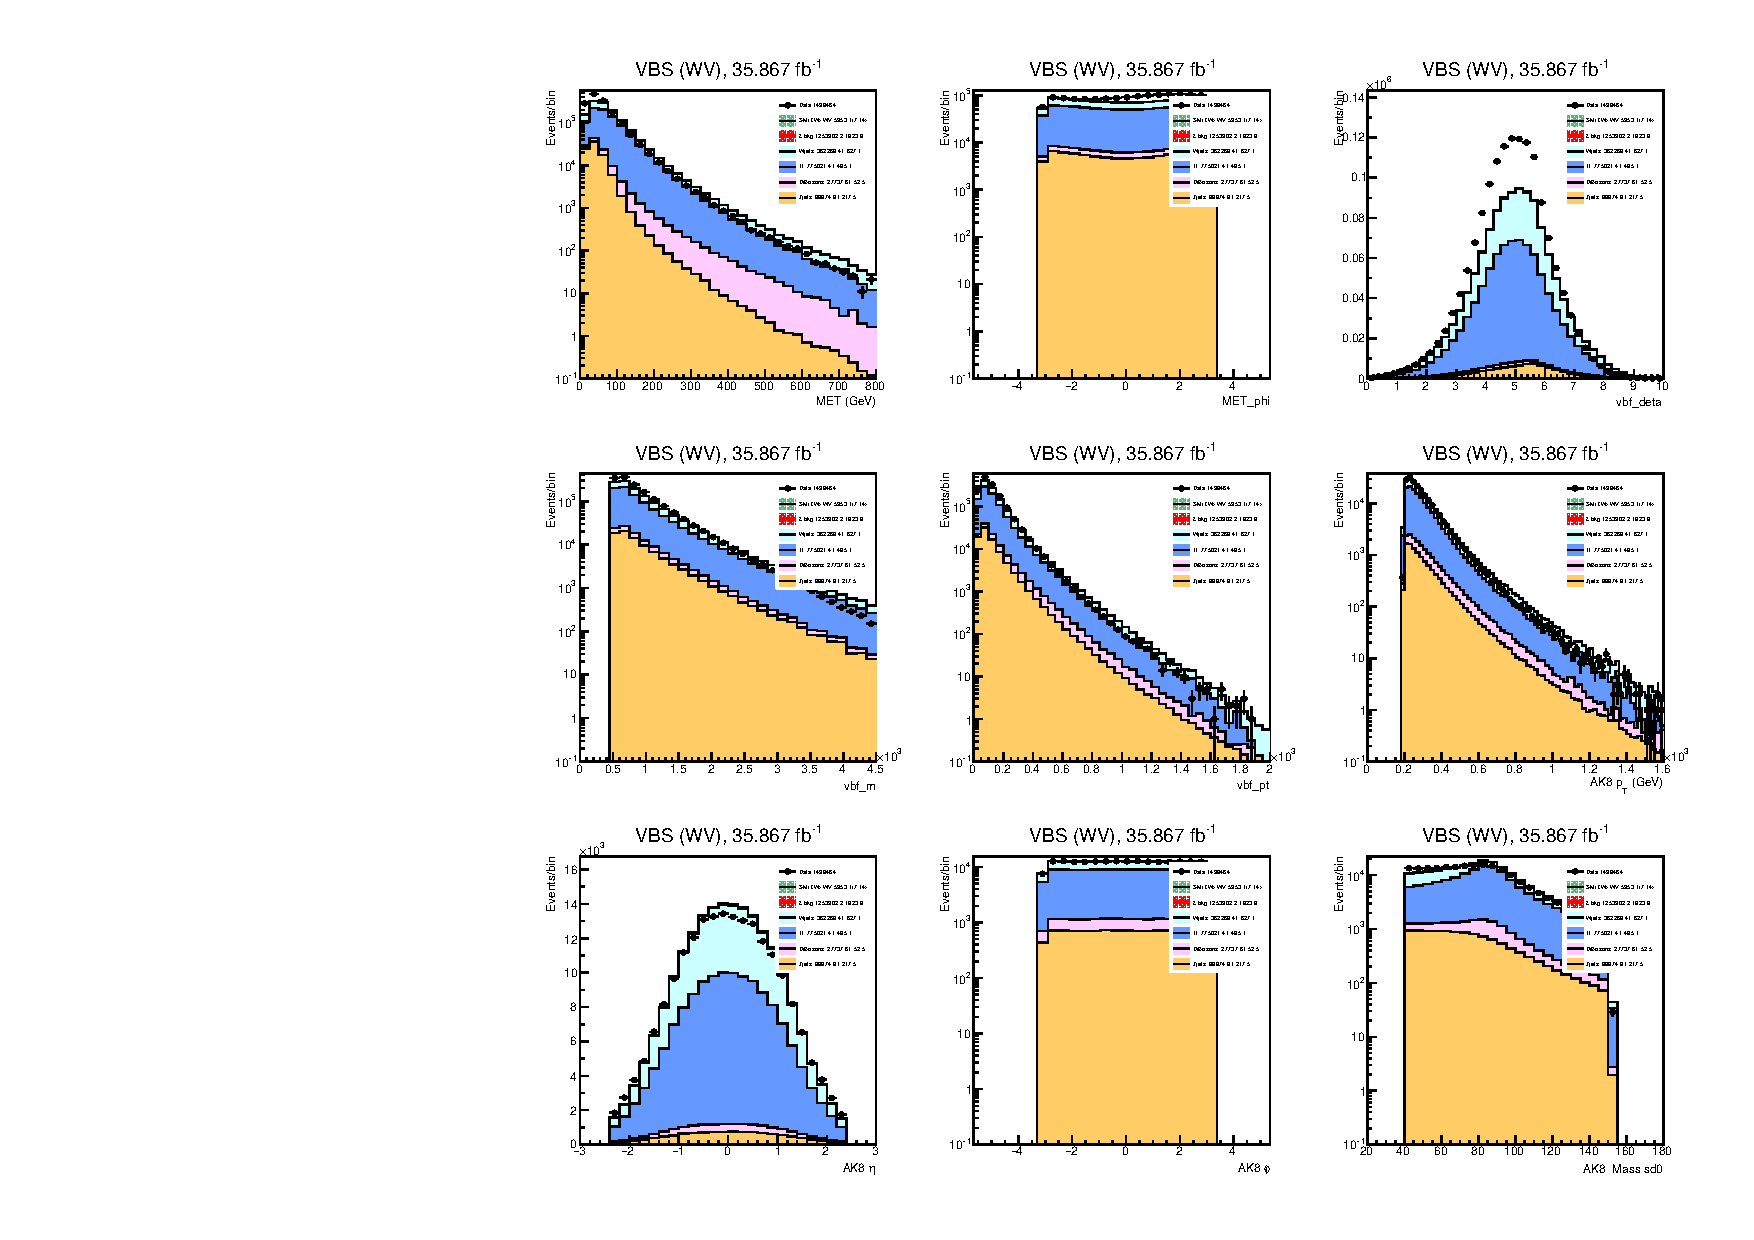
\includegraphics[width=\textwidth]{2016/c2_2016_test.pdf}
                \caption{2016 plot of c2 variables using cut: ``test"}
            \end{figure}
            \begin{figure}[H]
                \centering
                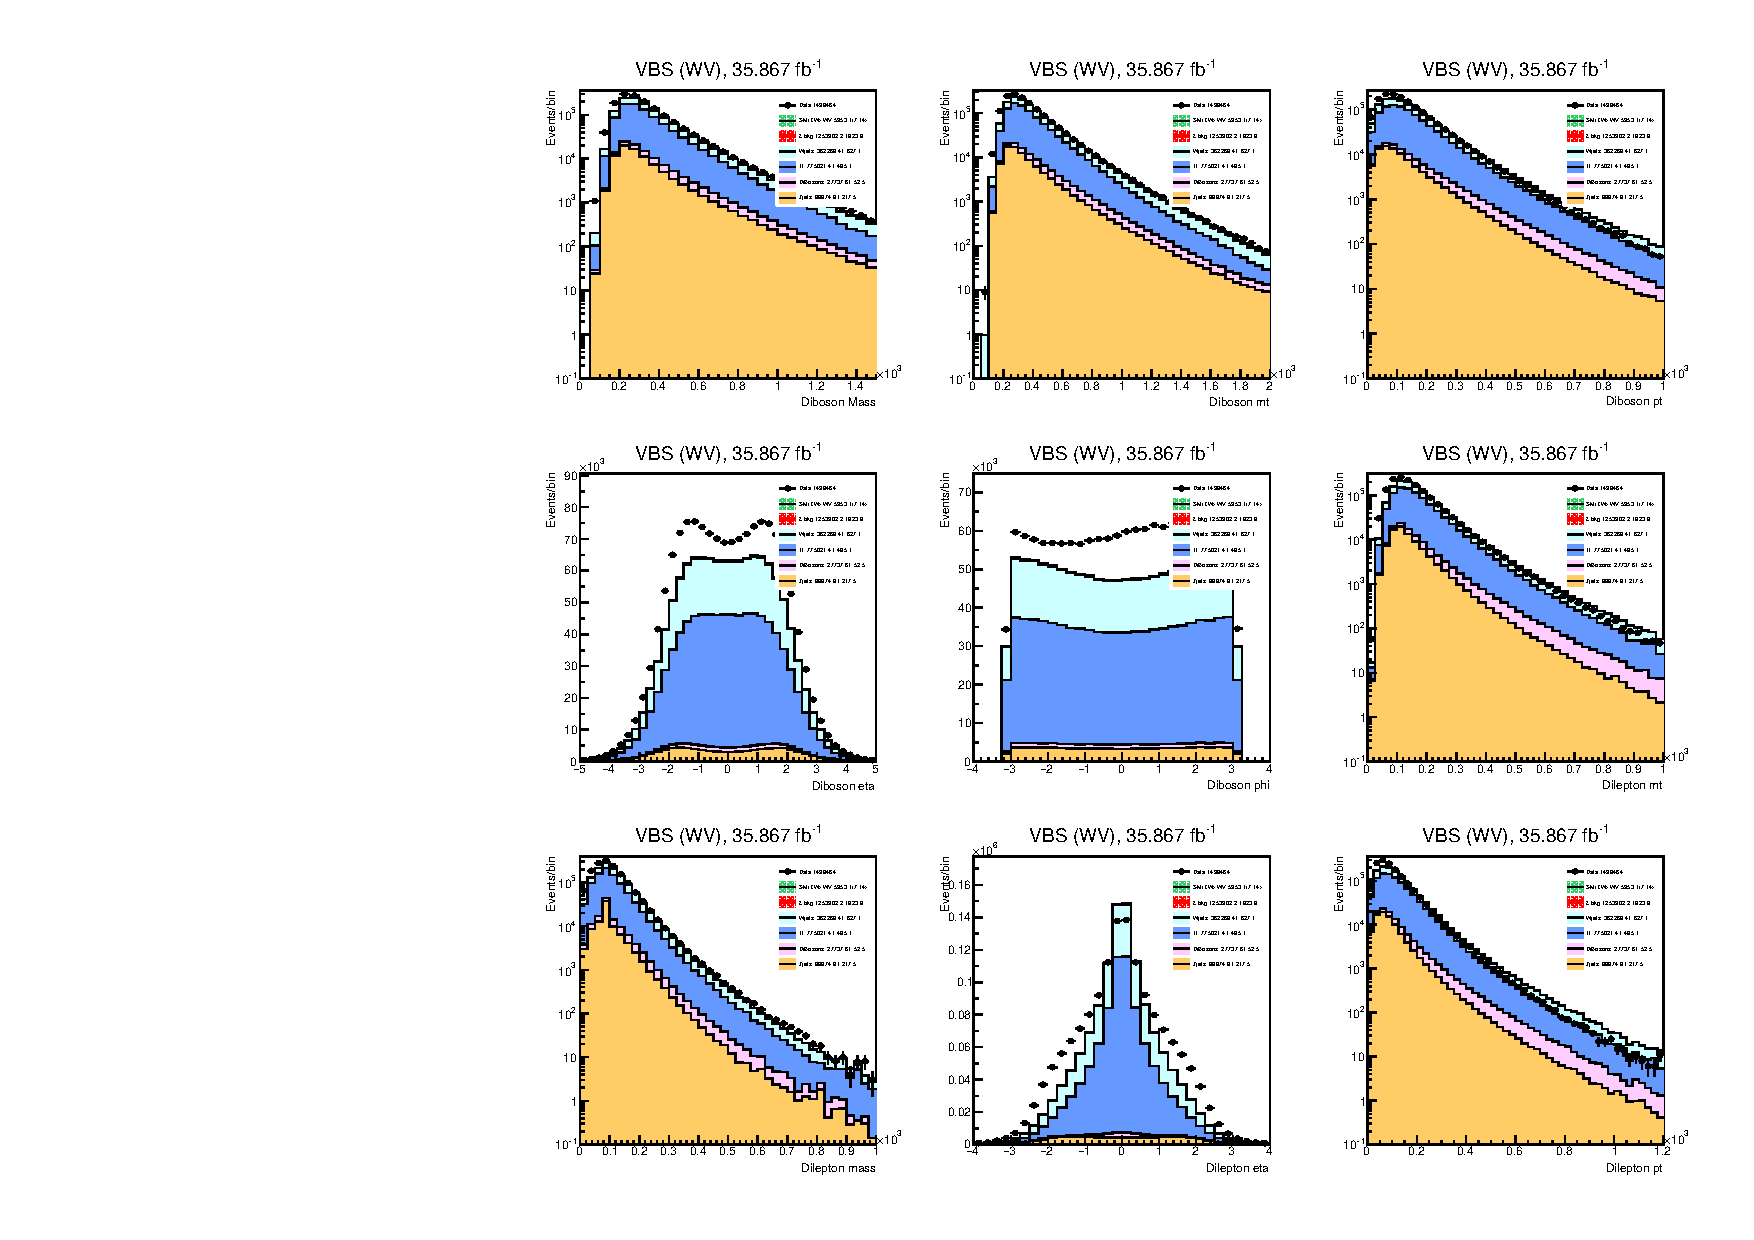
\includegraphics[width=\textwidth]{2016/c3_2016_test.pdf}
                \caption{2016 plot of c3 variables using cut: ``test"}
            \end{figure}
    \section*{2017}
      \subsection*{test}
            \begin{figure}[H]
                \centering
                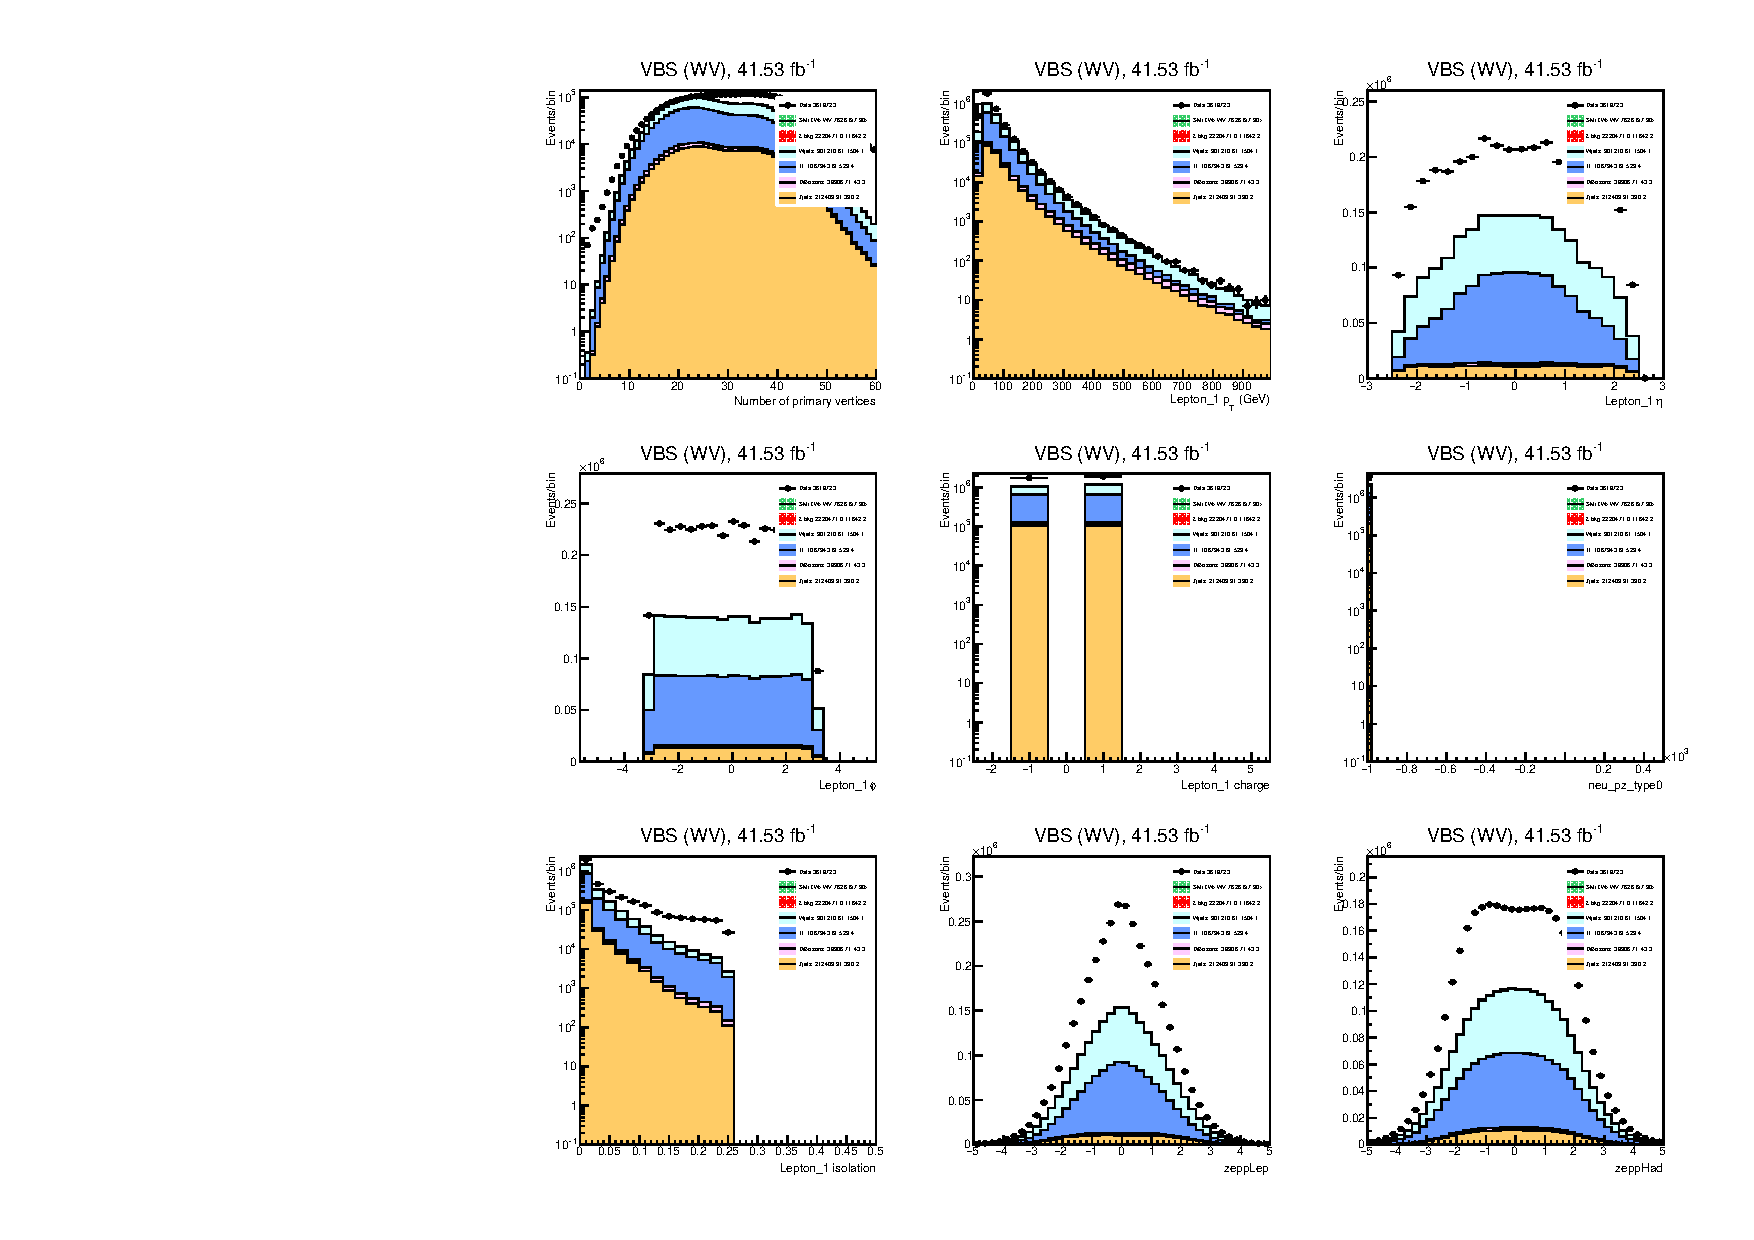
\includegraphics[width=\textwidth]{2017/c1_2017_test.pdf}
                \caption{2017 plot of c1 variables using cut: ``test"}
            \end{figure}
            \begin{figure}[H]
                \centering
                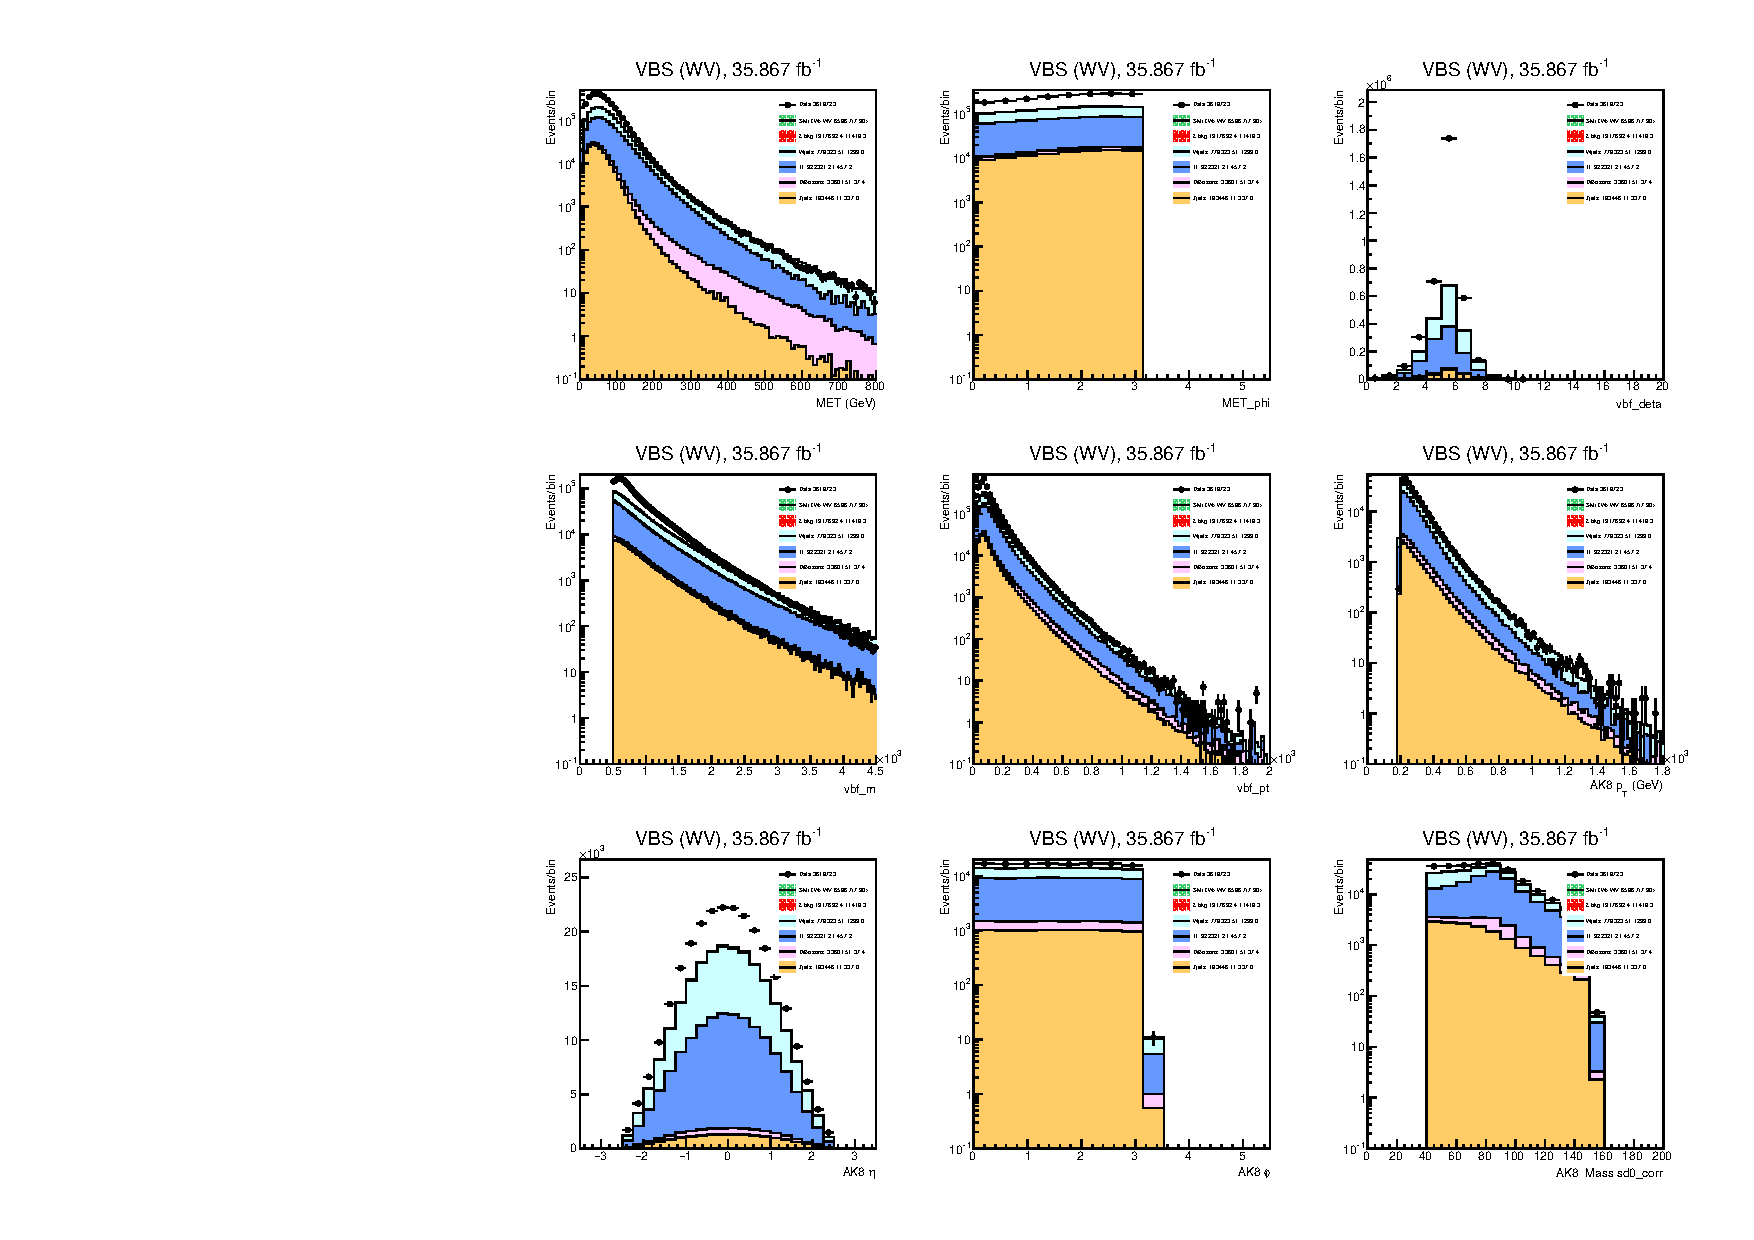
\includegraphics[width=\textwidth]{2017/c2_2017_test.pdf}
                \caption{2017 plot of c2 variables using cut: ``test"}
            \end{figure}
            \begin{figure}[H]
                \centering
                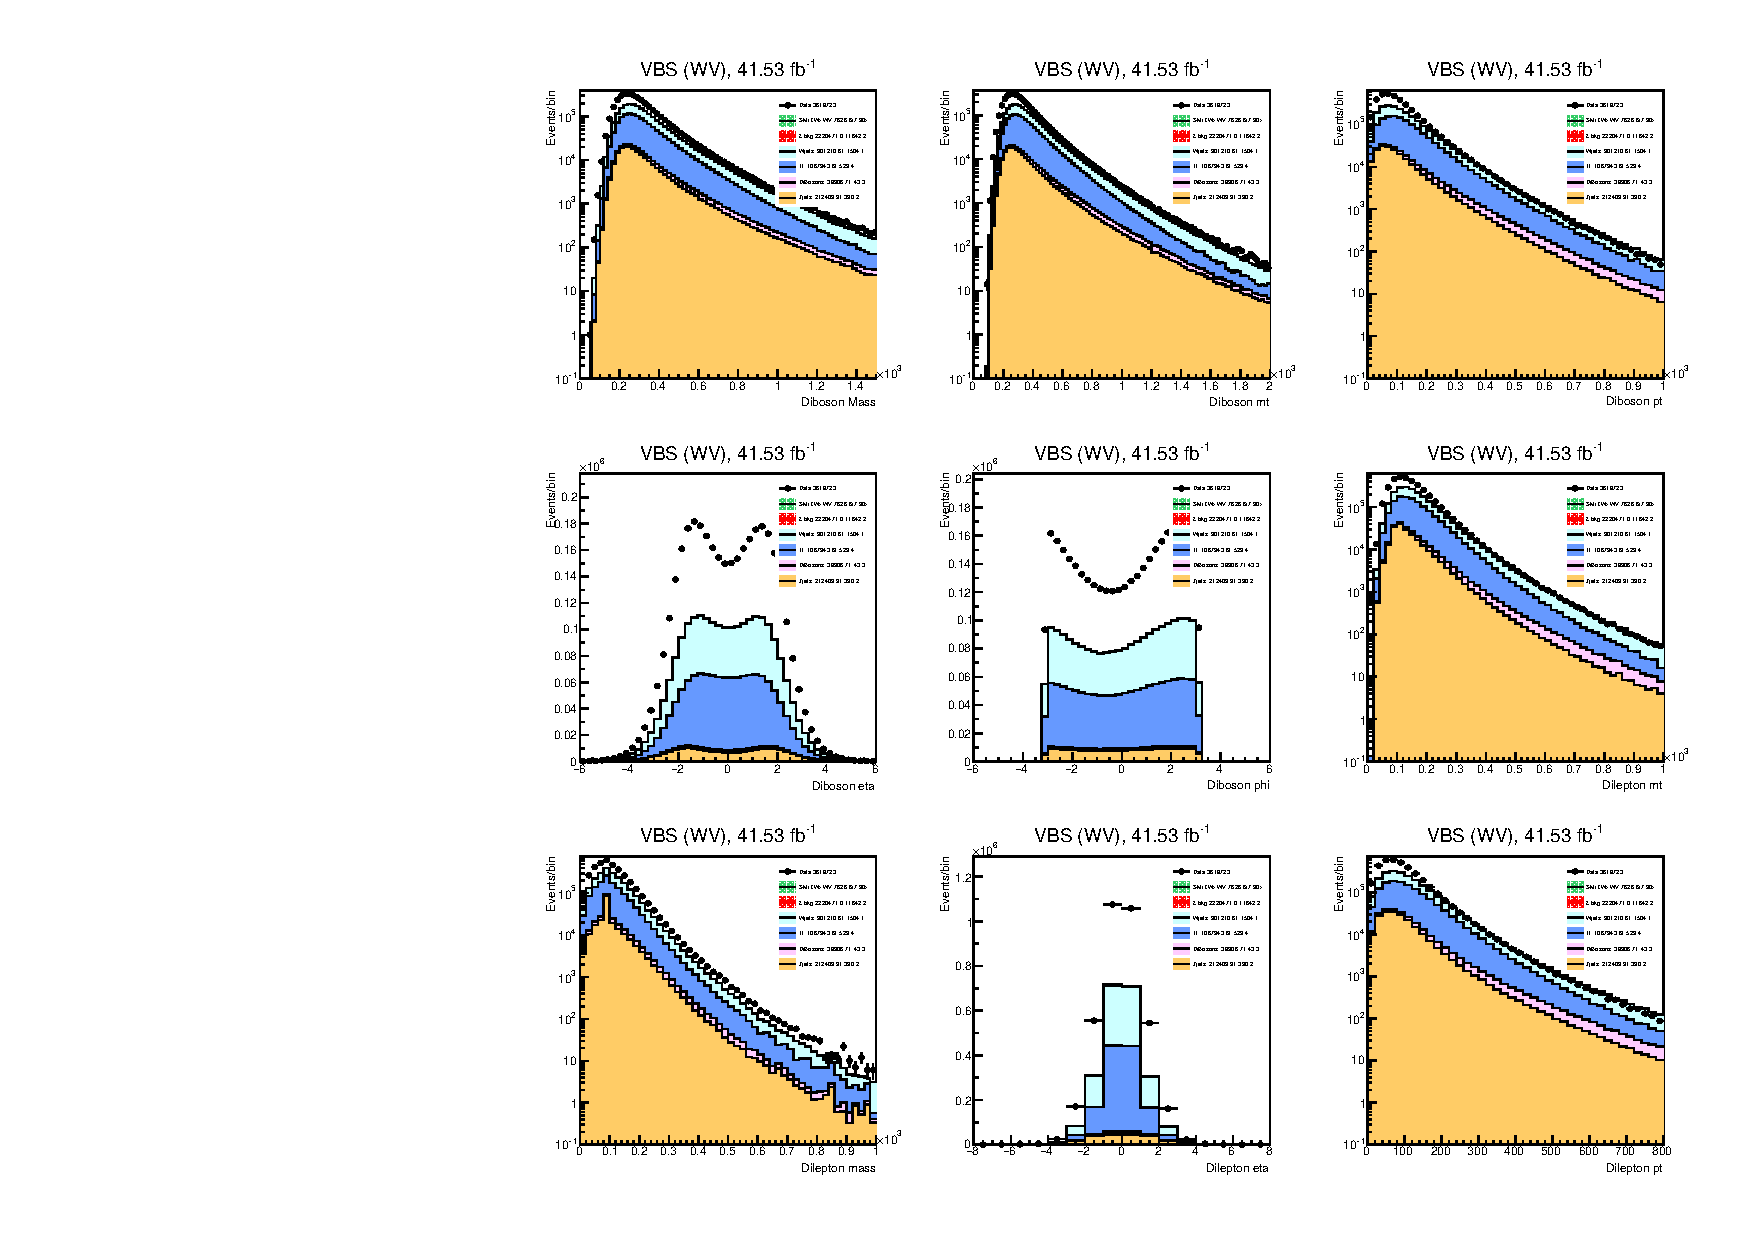
\includegraphics[width=\textwidth]{2017/c3_2017_test.pdf}
                \caption{2017 plot of c3 variables using cut: ``test"}
            \end{figure}
    \section*{2018}
      \subsection*{test}
            \begin{figure}[H]
                \centering
                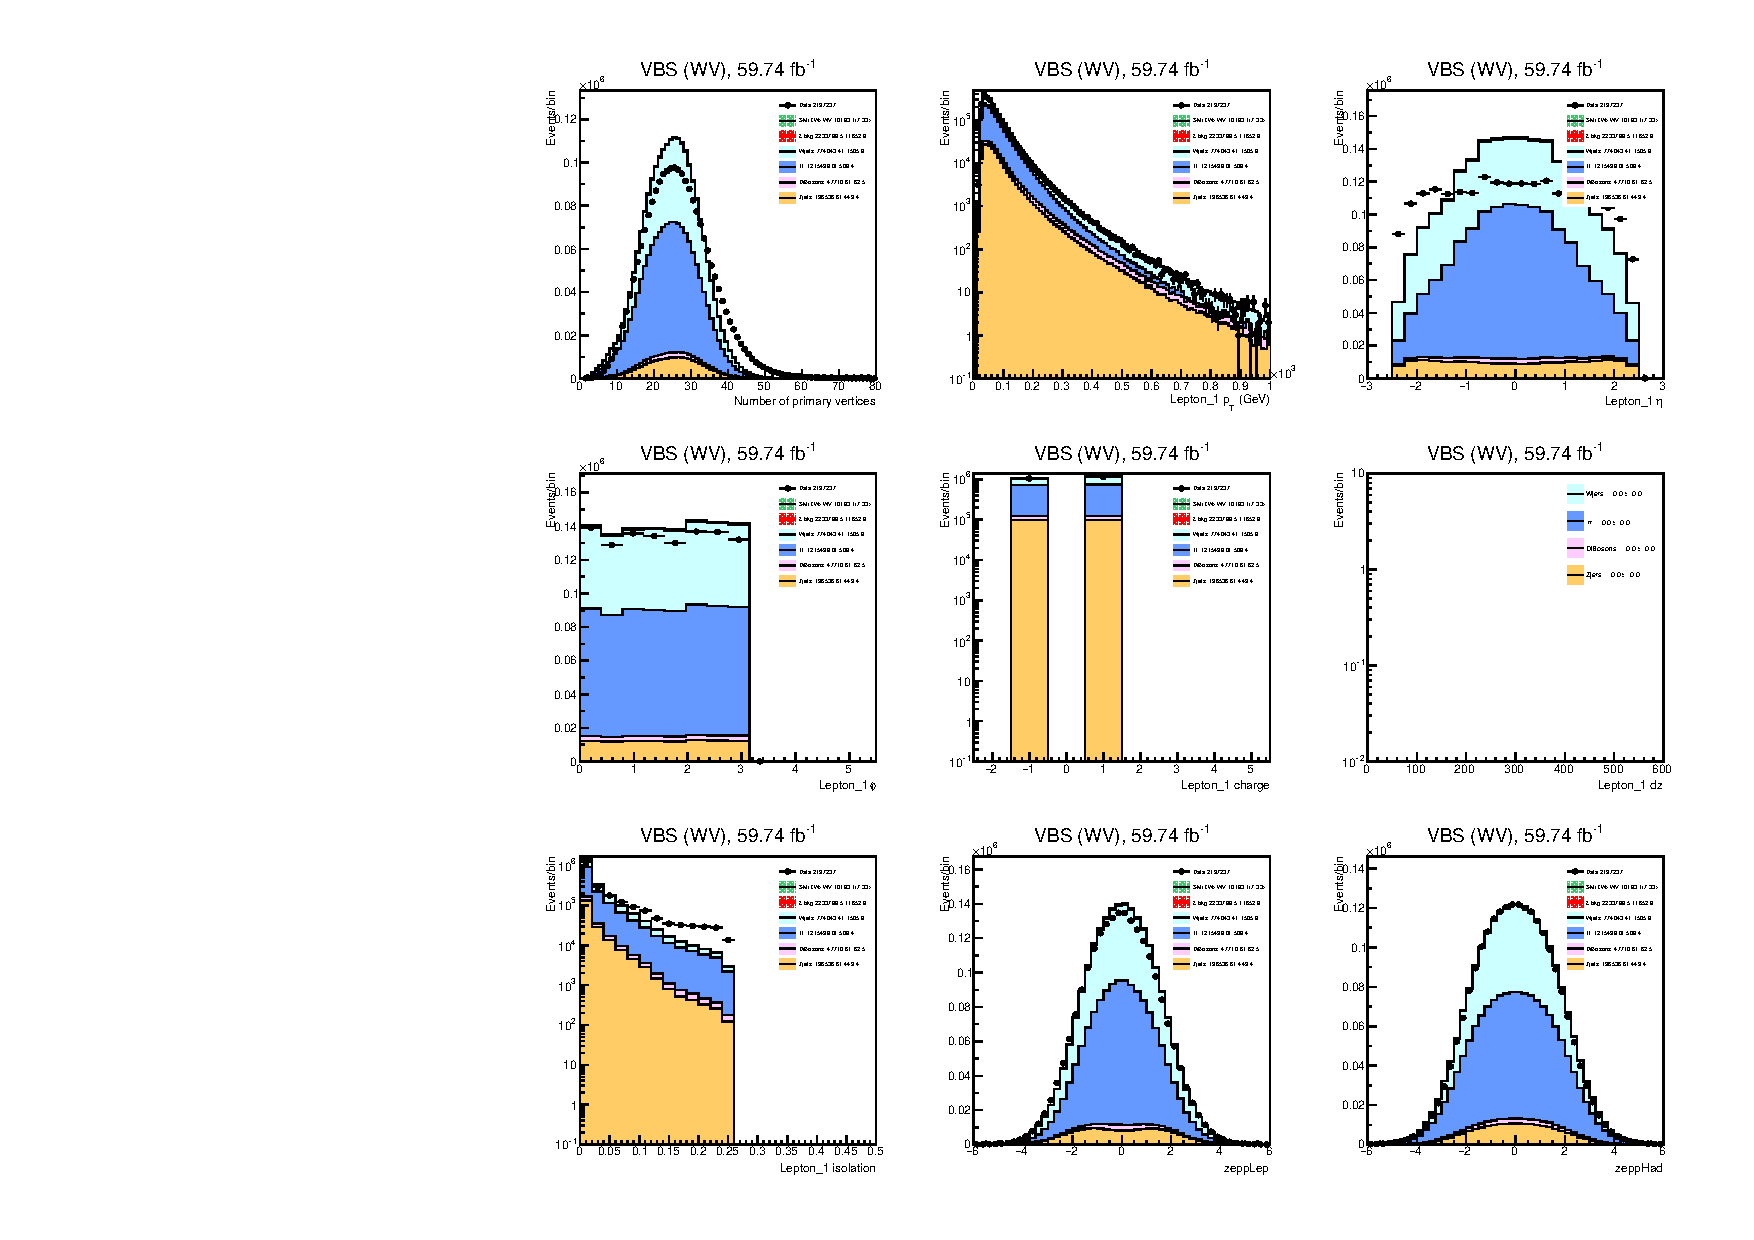
\includegraphics[width=\textwidth]{2018/c1_2018_test.pdf}
                \caption{2018 plot of c1 variables using cut: ``test"}
            \end{figure}
            \begin{figure}[H]
                \centering
                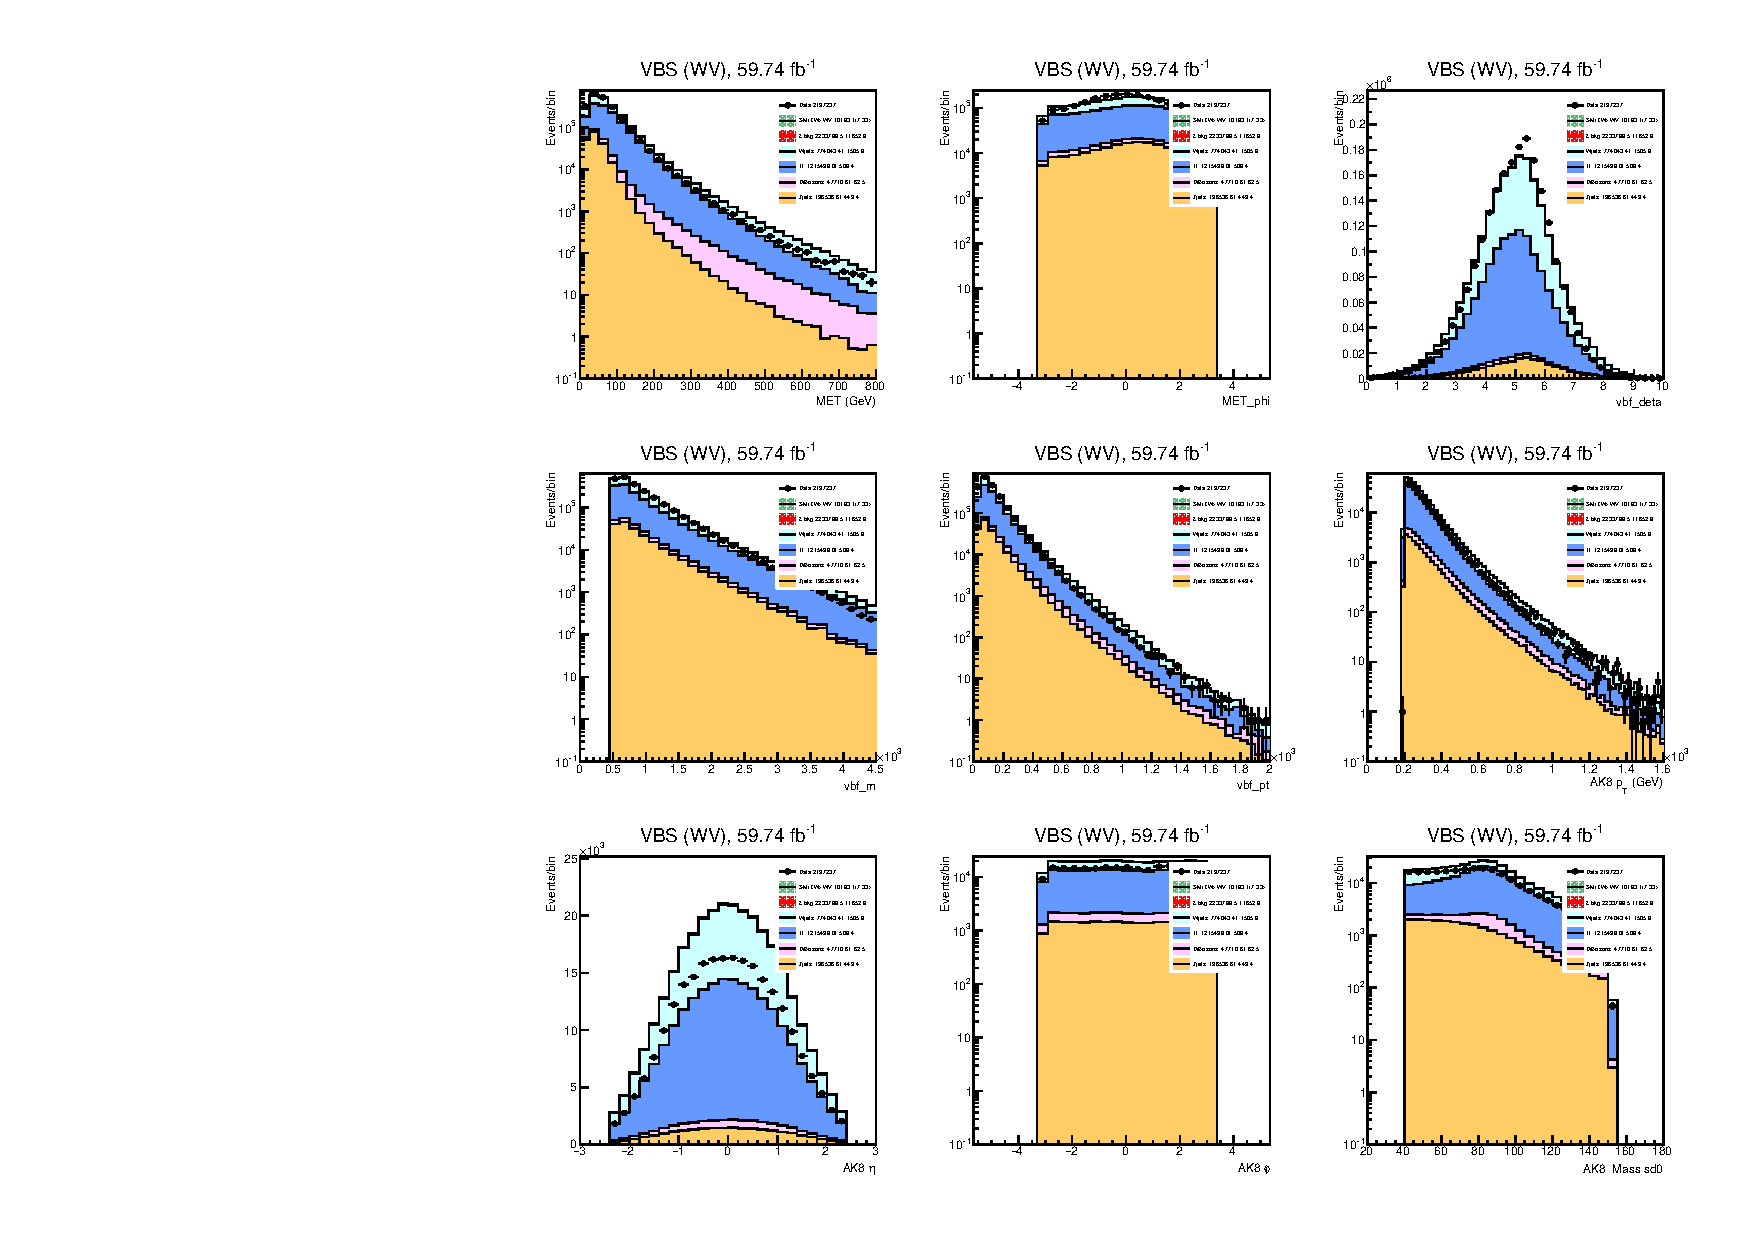
\includegraphics[width=\textwidth]{2018/c2_2018_test.pdf}
                \caption{2018 plot of c2 variables using cut: ``test"}
            \end{figure}
            \begin{figure}[H]
                \centering
                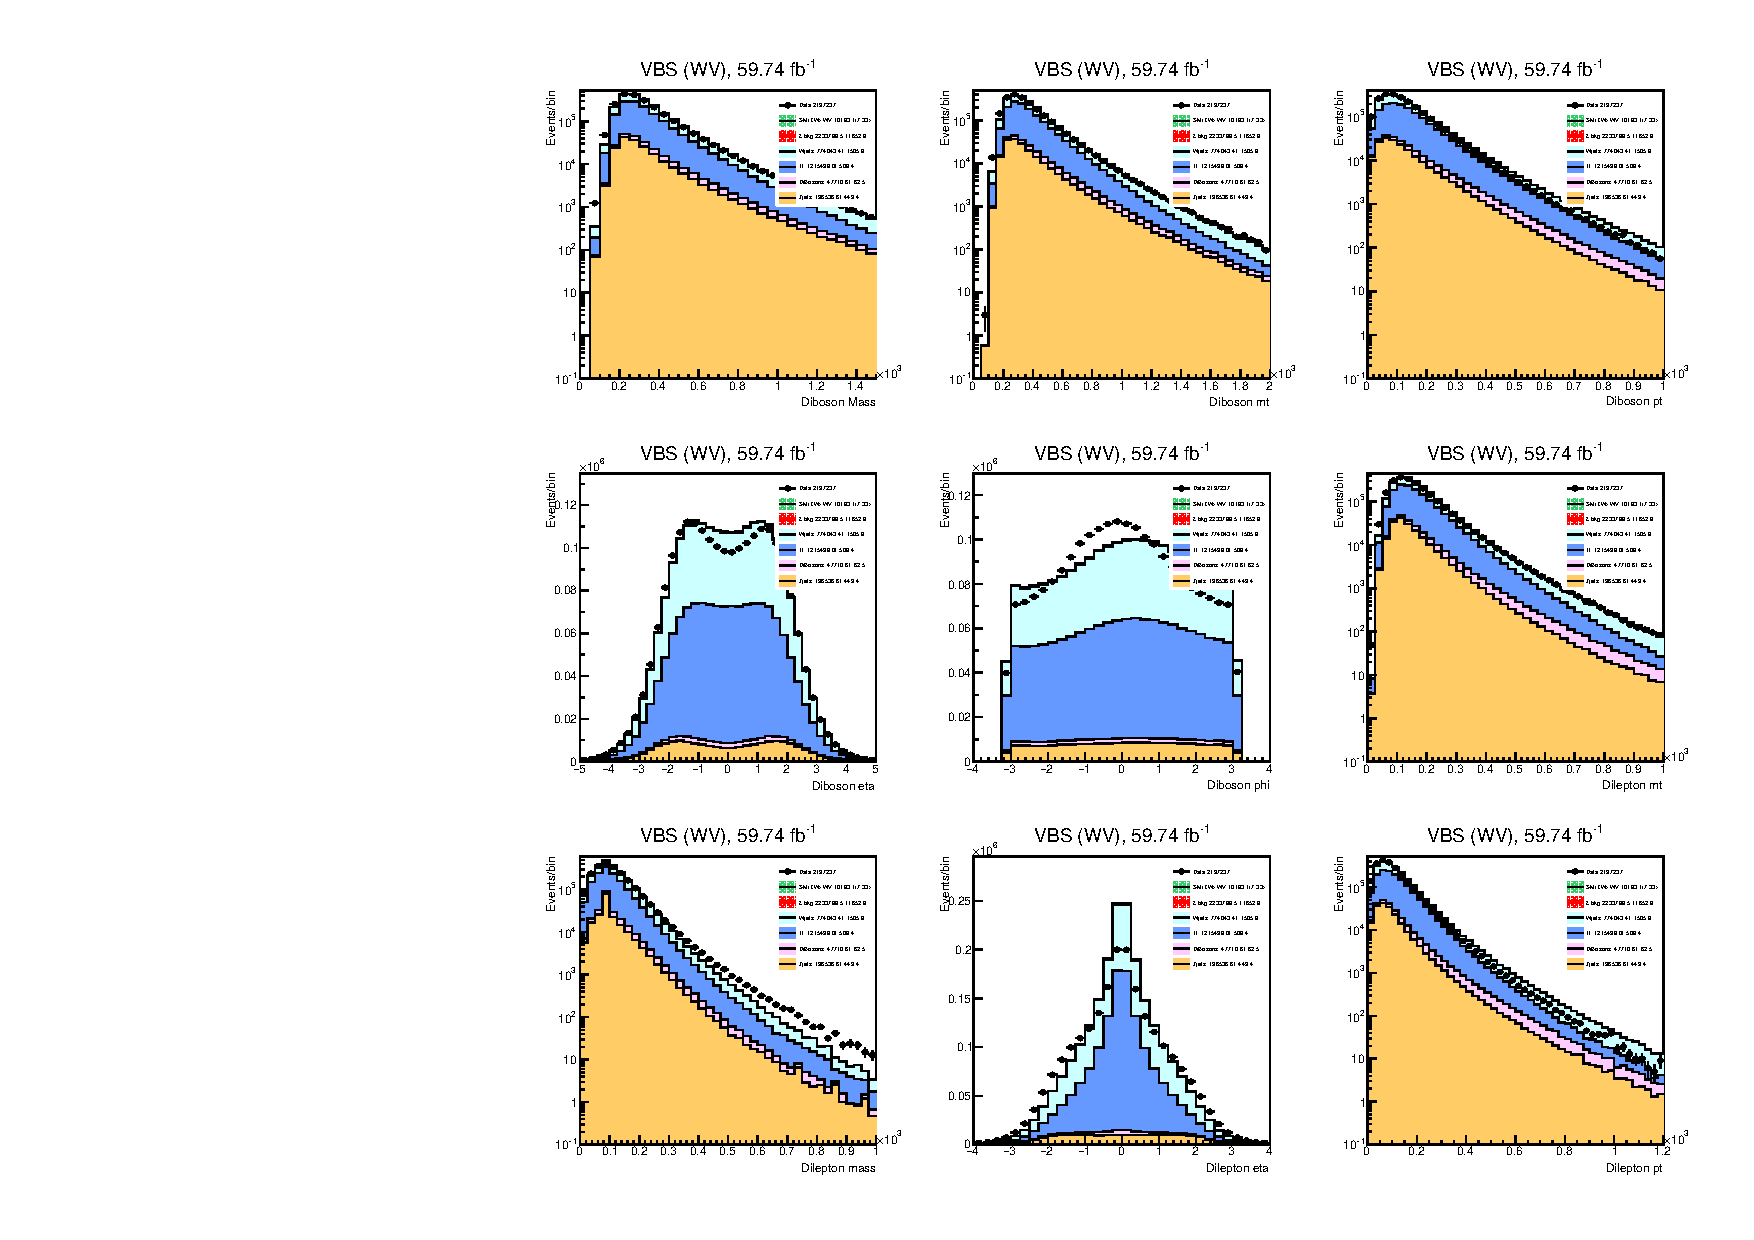
\includegraphics[width=\textwidth]{2018/c3_2018_test.pdf}
                \caption{2018 plot of c3 variables using cut: ``test"}
            \end{figure}
\end{document}
